\documentclass{standalone}
\usepackage{tikz}
\usetikzlibrary{patterns, positioning}
\usepackage[sfdefault]{ClearSans} %% option 'sfdefault' activates Clear Sans as the default text font
\usepackage[T1]{fontenc}

\begin{document}
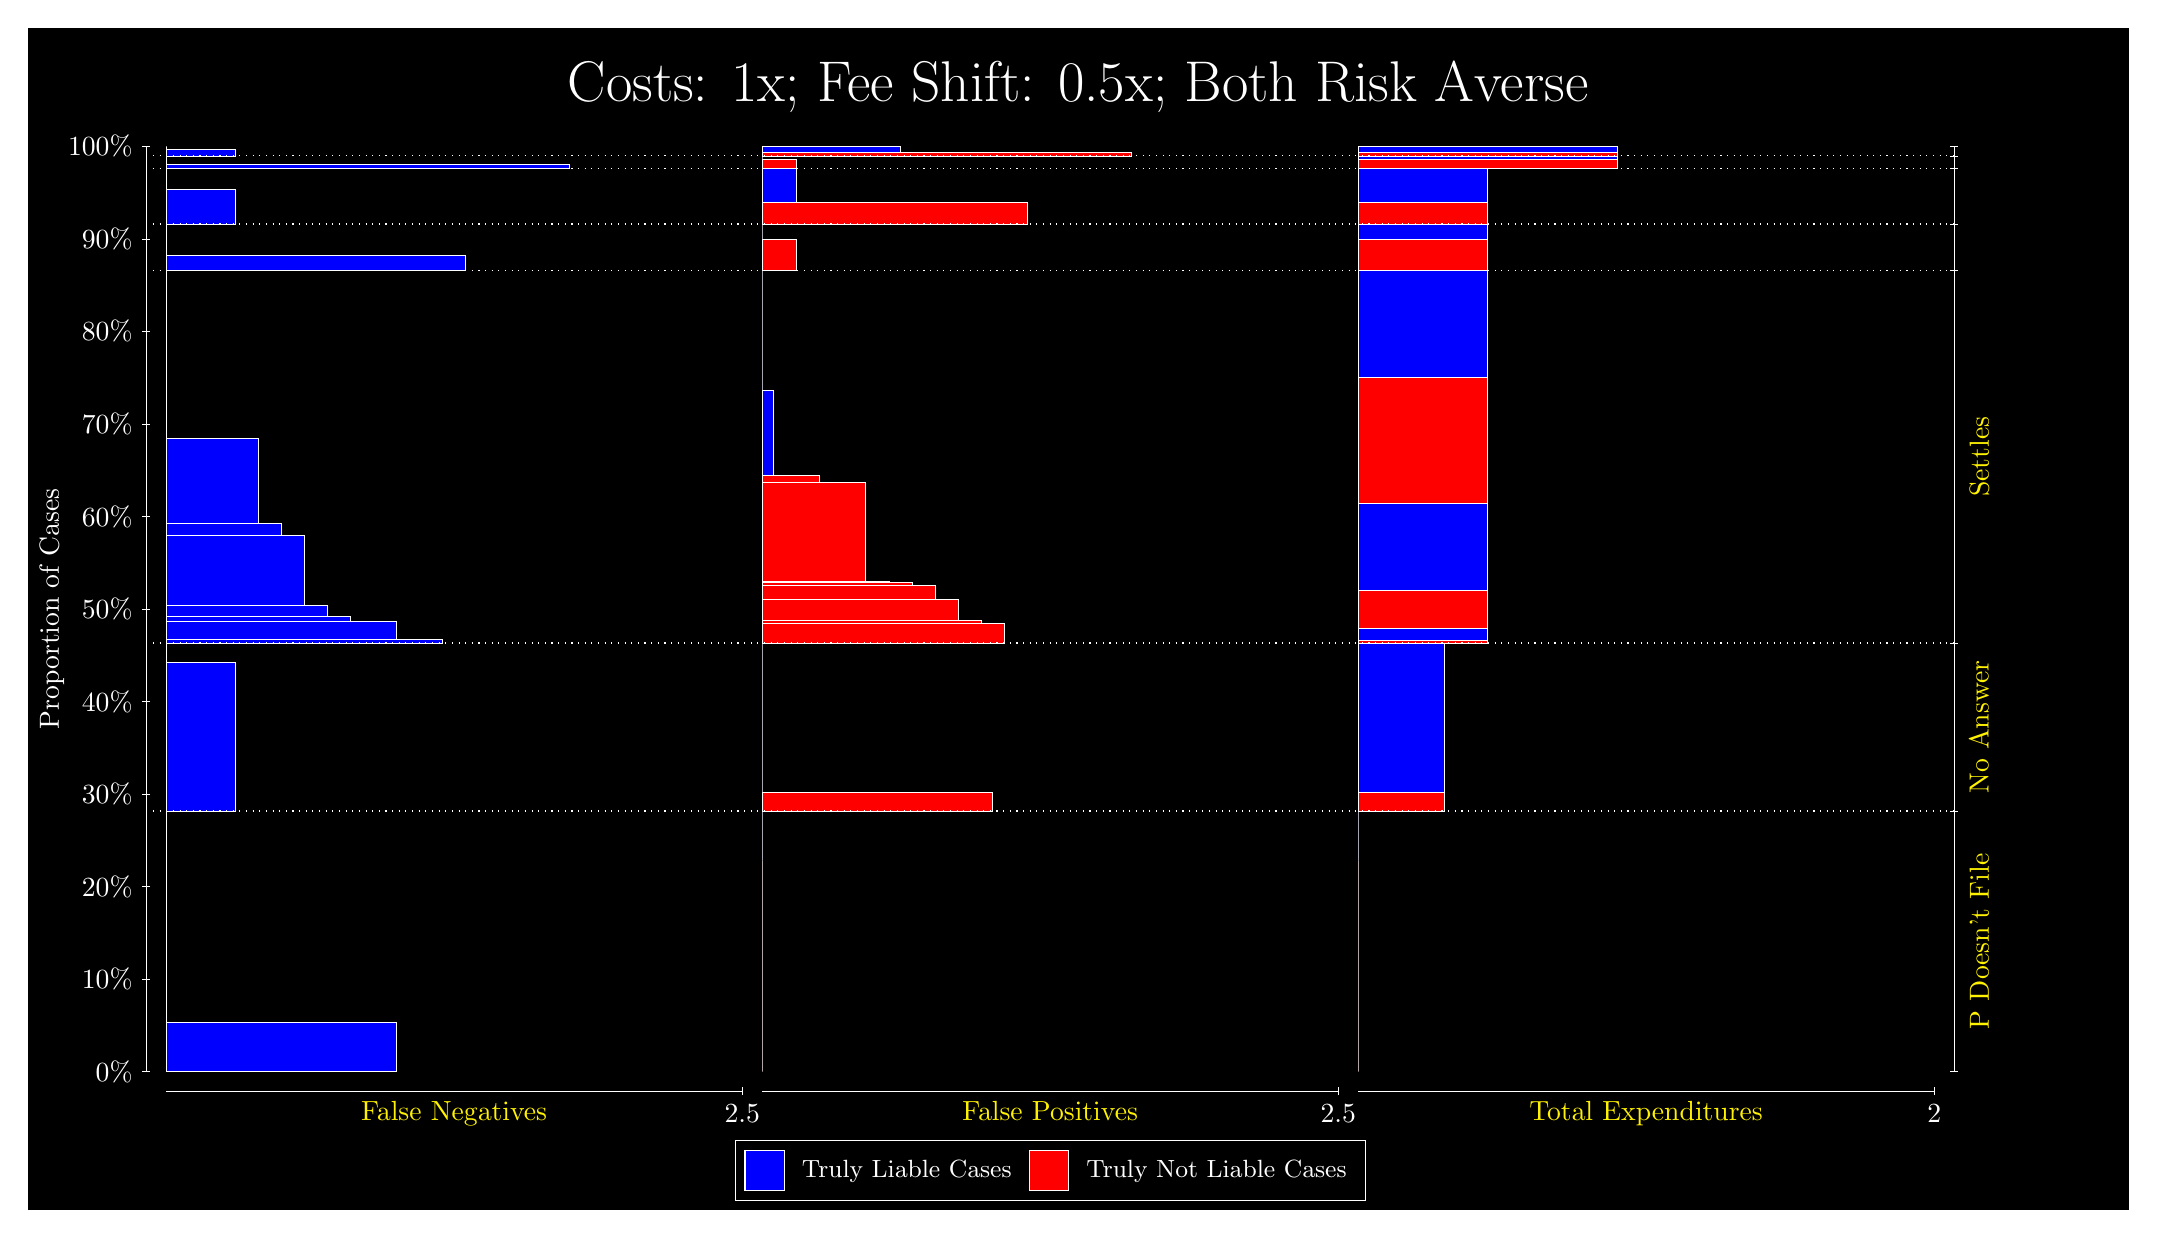
\begin{tikzpicture}
\draw[fill=black] (0,0) rectangle (26.667,15);
\draw[text=white] (0,13.5) rectangle (26.667,15) node[midway] {\huge Costs: 1x; Fee Shift: 0.5x; Both Risk Averse};
\draw[white, very thin] (1.5,1.75) -- (1.5,13.5);
\node[rotate=90, text=white, anchor=center] at (0.3, 7.625) {Proportion of Cases};
\draw[white, very thin] (1.45,1.75) -- (1.55,1.75);
\node[text=white, anchor=east] at (1.45, 1.75) {0\%};
\draw[white, very thin] (1.45,2.925) -- (1.55,2.925);
\node[text=white, anchor=east] at (1.45, 2.925) {10\%};
\draw[white, very thin] (1.45,4.1) -- (1.55,4.1);
\node[text=white, anchor=east] at (1.45, 4.1) {20\%};
\draw[white, very thin] (1.45,5.275) -- (1.55,5.275);
\node[text=white, anchor=east] at (1.45, 5.275) {30\%};
\draw[white, very thin] (1.45,6.45) -- (1.55,6.45);
\node[text=white, anchor=east] at (1.45, 6.45) {40\%};
\draw[white, very thin] (1.45,7.625) -- (1.55,7.625);
\node[text=white, anchor=east] at (1.45, 7.625) {50\%};
\draw[white, very thin] (1.45,8.8) -- (1.55,8.8);
\node[text=white, anchor=east] at (1.45, 8.8) {60\%};
\draw[white, very thin] (1.45,9.975) -- (1.55,9.975);
\node[text=white, anchor=east] at (1.45, 9.975) {70\%};
\draw[white, very thin] (1.45,11.15) -- (1.55,11.15);
\node[text=white, anchor=east] at (1.45, 11.15) {80\%};
\draw[white, very thin] (1.45,12.325) -- (1.55,12.325);
\node[text=white, anchor=east] at (1.45, 12.325) {90\%};
\draw[white, very thin] (1.45,13.5) -- (1.55,13.5);
\node[text=white, anchor=east] at (1.45, 13.5) {100\%};

\draw[white, very thin] (24.457,1.75) -- (24.457,13.5);
\draw[white, very thin] (24.407,1.75) -- (24.507,1.75);
\node[anchor=west] at (24.407, 1.75) {};
\draw[white, very thin] (24.407,5.0583) -- (24.507,5.0583);
\node[anchor=west] at (24.407, 5.0583) {};
\draw[white, very thin] (24.407,7.1927) -- (24.507,7.1927);
\node[anchor=west] at (24.407, 7.1927) {};
\draw[white, very thin] (24.407,11.922) -- (24.507,11.922);
\node[anchor=west] at (24.407, 11.922) {};
\draw[white, very thin] (24.407,12.513) -- (24.507,12.513);
\node[anchor=west] at (24.407, 12.513) {};
\draw[white, very thin] (24.407,13.223) -- (24.507,13.223);
\node[anchor=west] at (24.407, 13.223) {};
\draw[white, very thin] (24.407,13.378) -- (24.507,13.378);
\node[anchor=west] at (24.407, 13.378) {};
\draw[white, very thin] (24.407,13.5) -- (24.507,13.5);
\node[anchor=west] at (24.407, 13.5) {};

\draw[white, very thin, fill=blue] (1.75,1.75) rectangle (4.6775,2.3808);
\draw[white, very thin, fill=red] (1.75,2.3808) rectangle (1.75,5.0583);
\draw[white, very thin, fill=blue] (1.75,5.0583) rectangle (2.6283,6.9516);
\draw[white, very thin, fill=red] (1.75,6.9516) rectangle (1.75,7.1927);
\draw[white, very thin, fill=blue] (1.75,7.1927) rectangle (5.2631,7.2353);
\draw[white, very thin, fill=blue] (1.75,7.2353) rectangle (4.6775,7.4664);
\draw[white, very thin, fill=blue] (1.75,7.4664) rectangle (4.3848,7.4697);
\draw[white, very thin, fill=blue] (1.75,7.4697) rectangle (4.092,7.5269);
\draw[white, very thin, fill=blue] (1.75,7.5269) rectangle (3.7993,7.67);
\draw[white, very thin, fill=blue] (1.75,7.67) rectangle (3.5065,8.5658);
\draw[white, very thin, fill=blue] (1.75,8.5658) rectangle (3.2138,8.7115);
\draw[white, very thin, fill=blue] (1.75,8.7115) rectangle (2.921,9.7874);
\draw[white, very thin, fill=red] (1.75,9.7874) rectangle (1.75,11.922);
\draw[white, very thin, fill=blue] (1.75,11.922) rectangle (5.5558,12.12);
\draw[white, very thin, fill=red] (1.75,12.12) rectangle (1.75,12.513);
\draw[white, very thin, fill=blue] (1.75,12.513) rectangle (2.6283,12.949);
\draw[white, very thin, fill=red] (1.75,12.949) rectangle (1.75,13.223);
\draw[white, very thin, fill=blue] (1.75,13.223) rectangle (6.8732,13.266);
\draw[white, very thin, fill=red] (1.75,13.266) rectangle (1.75,13.378);
\draw[white, very thin, fill=blue] (1.75,13.378) rectangle (2.6283,13.457);
\draw[white, very thin, fill=red] (1.75,13.457) rectangle (1.75,13.5);
\draw[white, very thin, fill=red] (9.3189,1.75) rectangle (9.3189,4.4275);
\draw[white, very thin, fill=blue] (9.3189,4.4275) rectangle (9.3189,5.0583);
\draw[white, very thin, fill=red] (9.3189,5.0583) rectangle (12.246,5.2994);
\draw[white, very thin, fill=blue] (9.3189,5.2994) rectangle (9.3189,7.1927);
\draw[white, very thin, fill=red] (9.3189,7.1927) rectangle (12.393,7.4426);
\draw[white, very thin, fill=red] (9.3189,7.4426) rectangle (12.1,7.4796);
\draw[white, very thin, fill=red] (9.3189,7.4796) rectangle (11.807,7.744);
\draw[white, very thin, fill=red] (9.3189,7.744) rectangle (11.515,7.9215);
\draw[white, very thin, fill=red] (9.3189,7.9215) rectangle (11.222,7.9694);
\draw[white, very thin, fill=red] (9.3189,7.9694) rectangle (10.929,7.9727);
\draw[white, very thin, fill=red] (9.3189,7.9727) rectangle (10.636,9.2319);
\draw[white, very thin, fill=red] (9.3189,9.2319) rectangle (10.051,9.327);
\draw[white, very thin, fill=blue] (9.3189,9.327) rectangle (9.4652,10.403);
\draw[white, very thin, fill=blue] (9.3189,10.403) rectangle (9.3189,11.922);
\draw[white, very thin, fill=red] (9.3189,11.922) rectangle (9.758,12.315);
\draw[white, very thin, fill=blue] (9.3189,12.315) rectangle (9.3189,12.513);
\draw[white, very thin, fill=red] (9.3189,12.513) rectangle (12.686,12.787);
\draw[white, very thin, fill=blue] (9.3189,12.787) rectangle (9.758,13.223);
\draw[white, very thin, fill=red] (9.3189,13.223) rectangle (9.758,13.335);
\draw[white, very thin, fill=blue] (9.3189,13.335) rectangle (9.3189,13.378);
\draw[white, very thin, fill=red] (9.3189,13.378) rectangle (14.003,13.421);
\draw[white, very thin, fill=blue] (9.3189,13.421) rectangle (11.075,13.5);
\draw[white, very thin, fill=red] (16.888,1.75) rectangle (16.888,4.4275);
\draw[white, very thin, fill=blue] (16.888,4.4275) rectangle (16.888,5.0583);
\draw[white, very thin, fill=red] (16.888,5.0583) rectangle (17.986,5.2994);
\draw[white, very thin, fill=blue] (16.888,5.2994) rectangle (17.986,7.1927);
\draw[white, very thin, fill=red] (16.888,7.1927) rectangle (18.534,7.2298);
\draw[white, very thin, fill=blue] (16.888,7.2298) rectangle (18.534,7.3755);
\draw[white, very thin, fill=red] (16.888,7.3755) rectangle (18.534,7.8653);
\draw[white, very thin, fill=blue] (16.888,7.8653) rectangle (18.534,8.9614);
\draw[white, very thin, fill=red] (16.888,8.9614) rectangle (18.534,10.569);
\draw[white, very thin, fill=blue] (16.888,10.569) rectangle (18.534,11.922);
\draw[white, very thin, fill=red] (16.888,11.922) rectangle (18.534,12.315);
\draw[white, very thin, fill=blue] (16.888,12.315) rectangle (18.534,12.513);
\draw[white, very thin, fill=red] (16.888,12.513) rectangle (18.534,12.787);
\draw[white, very thin, fill=blue] (16.888,12.787) rectangle (18.534,13.223);
\draw[white, very thin, fill=red] (16.888,13.223) rectangle (20.181,13.335);
\draw[white, very thin, fill=blue] (16.888,13.335) rectangle (20.181,13.378);
\draw[white, very thin, fill=red] (16.888,13.378) rectangle (20.181,13.421);
\draw[white, very thin, fill=blue] (16.888,13.421) rectangle (20.181,13.5);
\draw[white, dotted] (1.5,5.0583) -- (24.457,5.0583);
\draw[white, dotted] (1.5,7.1927) -- (24.457,7.1927);
\draw[white, dotted] (1.5,11.922) -- (24.457,11.922);
\draw[white, dotted] (1.5,12.513) -- (24.457,12.513);
\draw[white, dotted] (1.5,13.223) -- (24.457,13.223);
\draw[white, dotted] (1.5,13.378) -- (24.457,13.378);
\draw[white, very thin] (1.75,1.5) -- (9.0689,1.5);
\node[text=yellow, anchor=north] at (5.4094, 1.5) {False Negatives};
\draw[white, very thin] (9.0689,1.45) -- (9.0689,1.55);
\node[text=white, anchor=north] at (9.0689, 1.45) {2.5};

\draw[white, very thin] (9.3189,1.5) -- (16.638,1.5);
\node[text=yellow, anchor=north] at (12.978, 1.5) {False Positives};
\draw[white, very thin] (16.638,1.45) -- (16.638,1.55);
\node[text=white, anchor=north] at (16.638, 1.45) {2.5};

\draw[white, very thin] (16.888,1.5) -- (24.207,1.5);
\node[text=yellow, anchor=north] at (20.547, 1.5) {Total Expenditures};
\draw[white, very thin] (24.207,1.45) -- (24.207,1.55);
\node[text=white, anchor=north] at (24.207, 1.45) {2};

\node[text=yellow, centered, rotate=90] at (24.777, 3.4042) {P Doesn't File};
\node[text=yellow, centered, rotate=90] at (24.777, 6.1255) {No Answer};
\node[text=yellow, centered, rotate=90] at (24.777, 9.5572) {Settles};





\draw (12.978300999999998,1.5) node[draw=none] (baseCoordinate) {};
\begin{scope}[align=center]
        \matrix[scale=0.5, draw=white, below=0.5cm of baseCoordinate, nodes={draw}, column sep=0.1cm]{
            \node[rectangle, draw, minimum width=0.5cm, minimum height=0.5cm, fill=blue] {}; &
            \node[draw=none, font=\small, text=white] (B) {Truly Liable Cases}; &
            \node[rectangle, draw, minimum width=0.5cm, minimum height=0.5cm, fill=red] {}; &
            \node[draw=none, font=\small, text=white] (B) {Truly Not Liable Cases}; \\
            };
\end{scope}

\end{tikzpicture}
\end{document}